
\documentclass[aspectratio=169,11pt]{beamer}
\usetheme{Madrid}
\setbeamertemplate{navigation symbols}{}
\setbeamertemplate{footline}[frame number]

\usepackage[T1]{fontenc}
\usepackage{lmodern}
\usepackage{amsmath,amssymb,booktabs,array,tikz,graphicx}
\usetikzlibrary{arrows.meta,positioning,fit,calc}

\definecolor{deepblue}{RGB}{27,70,129}
\definecolor{paleblue}{RGB}{235,242,250}
\definecolor{softgreen}{RGB}{222,242,231}

\setbeamercolor{structure}{fg=deepblue}
\setbeamercolor{block title}{bg=deepblue,fg=white}
\setbeamercolor{block body}{bg=paleblue,fg=black}

\newcommand{\key}[1]{\textcolor{deepblue}{\textbf{#1}}}
\newcommand{\figbox}[2]{\begin{center}\fcolorbox{deepblue}{paleblue}{\begin{minipage}[c][#1][c]{.89\linewidth}\centering\large\bfseries Figure placeholder\\[5pt]\normalsize\mdseries #2\end{minipage}}\end{center}}

\title[LLM Assessments and Decisions]{When Do LLM-Based Assessments Support Good Operational Decisions?}
\subtitle{A Discussion of Accuracy, Performance, and Robustness}
\author{Authors' names blinded for peer review}
\date{October 2026}

\begin{document}

\begin{frame}
\titlepage
\end{frame}

%------------------------------------------------
\begin{frame}{Why this question matters}

\begin{itemize}
\setlength{\itemsep}{10pt}

\item Operational models typically require \key{structured inputs} for resource-allocation decisions.

\item Much consequential organizational information is \key{unstructured}: clinical notes, incident reports, case descriptions, and service records.

\item LLMs can convert those narratives into assessments that enter decision models.

\item Yet an accurate assessment need not yield a \key{good operational decision}.

\end{itemize}

\begin{block}{Central concern}
What happens between the LLM assessment and the operational outcome---and which configurations perform reliably?
\end{block}

\end{frame}

%------------------------------------------------
\begin{frame}{The big picture: study the coupled system}

\begin{center}
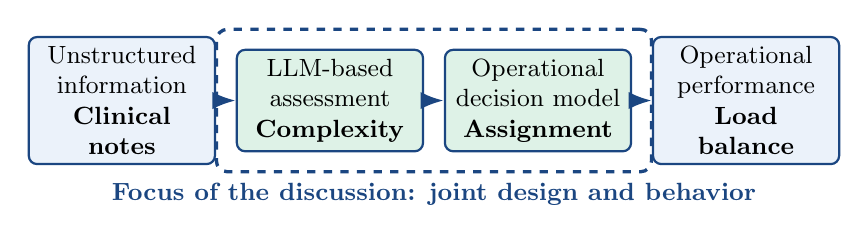
\begin{tikzpicture}[
node distance=.25cm,
>=Latex,
every node/.style={align=center}
]

\tikzset{
fbox/.style={
draw=deepblue,
thick,
rounded corners=3pt,
fill=paleblue,
minimum height=1.25cm,
text width=2.13cm,
font=\small
}
}

\node[fbox] (n) {
Unstructured\\
information\\
\textbf{Clinical notes}
};

\node[fbox,right=of n,fill=softgreen] (a) {
LLM-based\\
assessment\\
\textbf{Complexity}
};

\node[fbox,right=of a,fill=softgreen] (d) {
Operational\\
decision model\\
\textbf{Assignment}
};

\node[fbox,right=of d] (o) {
Operational\\
performance\\
\textbf{Load balance}
};

\draw[->,very thick,deepblue] (n)--(a);
\draw[->,very thick,deepblue] (a)--(d);
\draw[->,very thick,deepblue] (d)--(o);

\node[
draw=deepblue,
dashed,
very thick,
rounded corners,
fit=(a)(d),
inner sep=7pt,
label={[font=\small\bfseries,text=deepblue]below:Focus of the discussion: joint design and behavior}
] {};

\end{tikzpicture}
\end{center}

\vspace{.35cm}

\begin{block}{Experimental comparison}
Hold the \key{clinical-text inputs and patient groups fixed} when comparing how assessment configurations and decision policies interact. Vary operational settings deliberately and separately.
\end{block}

\end{frame}

%------------------------------------------------
\begin{frame}{Main questions discussed}

\small

\begin{enumerate}
\setlength{\itemsep}{9pt}

\item \key{Assessment accuracy:} How closely do LLM assessments agree with reference assessments?

\item \key{Operational performance:} Do more accurate assessments necessarily yield better allocations?

\item \key{Outcome robustness:} How do outcomes vary across optimal assignments, starting conditions, and client groups?

\item \key{Uncertainty-aware decisions:} What changes when LLM-reported probabilities enter a scenario-based decision model rather than a point-estimate model?

\item \key{Decision-aware inference (discussion direction):} Can an LLM's inference be partially or fully tailored to the downstream decision problem?

\end{enumerate}

\end{frame}

%------------------------------------------------
\begin{frame}{Working example: pediatric rehabilitation caseload assignment}

\begin{columns}[T,onlytextwidth]

\begin{column}{.49\textwidth}

\begin{block}{Inputs}
\begin{itemize}
\setlength{\itemsep}{5pt}

\item Pre-treatment notes (held fixed across compared models)

\item Client complexity inferred from notes

\item Existing clinician workloads

\item Maximum number of clients per clinician and other feasibility restrictions

\end{itemize}
\end{block}

\end{column}

\begin{column}{.48\textwidth}

\begin{block}{Decision}
Assign incoming clients to clinicians to balance resulting \key{total complexity workload}, while respecting assignment and client-count restrictions.
\end{block}

\end{column}

\end{columns}

\vspace{.2cm}

\begin{center}
\large
Clinical text $\rightarrow$ complexity assessment $\rightarrow$ allocation $\rightarrow$ workload balance
\end{center}

\begin{alertblock}{Scope}
Caseload assignment is a working example for studying the text-to-decision pipeline, not evidence of clinical deployment effectiveness.
\end{alertblock}

\end{frame}

%------------------------------------------------
\begin{frame}{Assignment model: only the essential structure}

\begin{columns}[T,onlytextwidth]

\begin{column}{.51\textwidth}

\begin{itemize}
\setlength{\itemsep}{8pt}

\item $x_{ij}=1$ if client $i$ is assigned to clinician $j$.

\item $s_i$: assessed client complexity.

\item $H_j$: clinician $j$'s initial complexity load.

\item Resulting load:
\vspace{-7pt}

\[
W_j(x;s)=H_j+\sum_i s_i x_{ij}.
\]

\end{itemize}

\end{column}

\begin{column}{.46\textwidth}

\begin{block}{Feasible assignments}

\begin{itemize}
\setlength{\itemsep}{5pt}

\item Each incoming client is assigned once.

\item Each clinician's allowed client count is respected.

\item Other assignment restrictions remain the same across comparisons.

\end{itemize}

\end{block}

\end{column}

\end{columns}

\begin{block}{Operational loss: complexity range}

\[
F(x;s,\theta)=\max_j W_j(x;s)-\min_j W_j(x;s).
\]

\vspace{-6pt}

\small
Here $\theta$ collects starting loads and constraints; lexicographic priorities, if present, are handled within each optimization model.

\end{block}

\end{frame}

%------------------------------------------------
\begin{frame}{From LLM assessments to decision regret}

\begin{itemize}
\setlength{\itemsep}{8pt}

\item The decision system selects an allocation $x=D(\hat s;\theta)$ from LLM assessments $\hat s$.

\item Evaluate $x$ using \key{reference assessments} $s^{\mathrm{ref}}$ under the \key{same} operational conditions.

\end{itemize}

\[
V^{\mathrm{ref}}(\theta)
=
\min_{y\in\mathcal X(\theta)}
F(y;s^{\mathrm{ref}},\theta)
\]

\[
\boxed{
R(x)=F(x;s^{\mathrm{ref}},\theta)-V^{\mathrm{ref}}(\theta)
}
\]

\begin{block}{Interpretation}
Regret is the additional workload imbalance relative to the reference-information optimum. Reference labels evaluate the allocation; they do not generate the LLM-based decision.
\end{block}

\end{frame}

%------------------------------------------------
\begin{frame}{Three distinct lenses on the same system}

\begin{columns}[T,onlytextwidth]

\begin{column}{.32\textwidth}

\begin{block}{Accuracy}
\small
Agreement between LLM and reference labels.

\vspace{6pt}

Exact accuracy and quadratic-weighted $\kappa$.
\end{block}

\end{column}

\begin{column}{.32\textwidth}

\begin{block}{Performance}
\small
Cost of the resulting allocation.

\vspace{6pt}

Reference-evaluated regret and workload imbalance.
\end{block}

\end{column}

\begin{column}{.32\textwidth}

\begin{block}{Robustness of outcomes}
\small
\textbf{Distribution and variation} of regret and assignments across tested conditions.

\vspace{6pt}

Compare centers, spread, and outliers.
\end{block}

\end{column}

\end{columns}

\vspace{.35cm}

\centering
\key{An accurate assessment need not yield a stable or high-performing decision.}

\end{frame}

%------------------------------------------------
\begin{frame}{Where do differences in outcomes come from?}

\begin{enumerate}
\setlength{\itemsep}{12pt}

\item \key{Patient groups (chunks):} Different mixes of incoming clients.

\item \key{Starting clinician profiles:} Balanced, unbalanced, and highly unbalanced loads.

\item \key{Multiple optimal assignments:} Different allocations with equal modeled objective value, potentially different reference regret.

\iffalse
\item \key{LLM probability distributions:} An additional input to \emph{scenario-based stochastic programming}, distinct from solver-selection randomness.
\fi

\end{enumerate}

\begin{block}{Comparison principle}
Keep these sources separate where possible; a solver seed is not a probability scenario or an independently sampled patient population.
\end{block}

\end{frame}

%------------------------------------------------
\begin{frame}{How LLM inference enters the decision model}

\begin{columns}[T,onlytextwidth]

\begin{column}{.48\textwidth}

\begin{block}{Deterministic input}

\begin{itemize}
\setlength{\itemsep}{6pt}

\item LLM provides one complexity category per client.

\item With class probabilities, select the \key{highest-probability class} (argmax).

\item Optimize the assignment using these point assessments.

\end{itemize}

\end{block}

\end{column}

\begin{column}{.48\textwidth}

\begin{block}{Stochastic input}

\begin{itemize}
\setlength{\itemsep}{6pt}

\item LLM reports probabilities for the complexity classes.

\item Use those probabilities to generate possible complexity profiles.

\item Choose \key{one allocation} with good average performance across sampled profiles.

\end{itemize}

\end{block}

\end{column}

\end{columns}

\vspace{.3cm}

\begin{alertblock}{Interpretation}
The difference lies in \key{how LLM inference is represented and used} by the downstream model, not in changing the original clinical notes.
\end{alertblock}

\end{frame}

%------------------------------------------------
\begin{frame}{A unified experimental design}

\footnotesize

\renewcommand{\arraystretch}{1.47}

\begin{tabular}{p{.27\linewidth}p{.64\linewidth}}

\toprule

\textbf{Dimension} & \textbf{Design} \\

\midrule

LLM configuration &
Qwen, MedGemma, and OpenDecider; compare prompting settings and self-reported confidence where available \\

Decision policy &
Deterministic point-assessment versus scenario-based stochastic \\

Client composition &
Common patient chunks for matched comparisons \\

Initial conditions &
Balanced, unbalanced, highly unbalanced clinician loads; common count constraints \\

Solution selection &
Different valid optimal assignments / solver selection seeds \\

Reference evaluation &
\textbf{Proxy benchmark} used consistently to score regret; clinician labels where fully available \\

\bottomrule

\end{tabular}

\vspace{.23cm}

\begin{center}
\key{Analyze the resulting distributions of regret and assignments under comparable conditions.}
\end{center}

\end{frame}

\iffalse
%------------------------------------------------
\begin{frame}{How results will be displayed: distributions, not a single score}

\begin{itemize}
\setlength{\itemsep}{10pt}

\item \key{Boxplots of regret} across models, chunks, starting profiles, and sampled optimal assignments.

\item Compare medians, interquartile ranges, whiskers, and visible outliers---alongside individual points where informative.

\item Display \key{assignment variation} separately, because different allocations can have similar regret.

\end{itemize}


\end{frame}
\fi
%------------------------------------------------
\begin{frame}{Analysis I: assessment accuracy versus decision quality}

\figbox{1.7cm}{Accuracy / agreement versus regret(And also assignment) distributions scatters}

\end{frame}

%------------------------------------------------
\begin{frame}{Decision/Performance Distributions Across Uncertainty Sources}


\figbox{1.8cm}{Regret(and also Assignment) boxplots by LLM and decision policy, with an assignment-comparison panel.}

\end{frame}

%------------------------------------------------
\begin{frame}{Analysis III: context dependence and assignment variability}

\begin{itemize}
\setlength{\itemsep}{9pt}

\item Repeat comparisons across \key{balanced, unbalanced, and highly unbalanced} starting workloads.

\item Hold client chunks fixed when isolating the influence of initial clinician loads.

\item Include variation due to alternative \key{equally optimal allocations} in the displayed distributions.

\item Ask whether the preferred LLM--decision combination changes with the operating environment.

\end{itemize}

\figbox{1.8cm}{Regret and assignment boxplots faceted by chunk and starting workload profile.}

\end{frame}

%------------------------------------------------
\begin{frame}{Conclusions}

\begin{enumerate}
\setlength{\itemsep}{10pt}

\item \key{Assessment--decision disconnect:} similar prediction quality, different regret.

\item \key{Context-dependent rankings:} different preferred LLM--decision combinations under different clinician loads.

\item \key{Solution-selection sensitivity:} identical modeled optimality, different reference outcomes.

\item \key{Uncertain inference:} when full class probabilities change allocation behavior compared with top-class labels.

\item \key{Decision-aware inference:} might information extraction itself be tailored to the downstream allocation task?

\end{enumerate}

\vspace{.1cm}

\small
\textit{These are questions for analysis, not established empirical findings.}

\end{frame}


\begin{frame}{Next Possible Steps}
    
\end{frame}


\end{document}
